\documentclass[varwidth=true, border=2pt]{standalone}

\usepackage{pgfplots}
\usepackage{tikz}

\begin{document}
	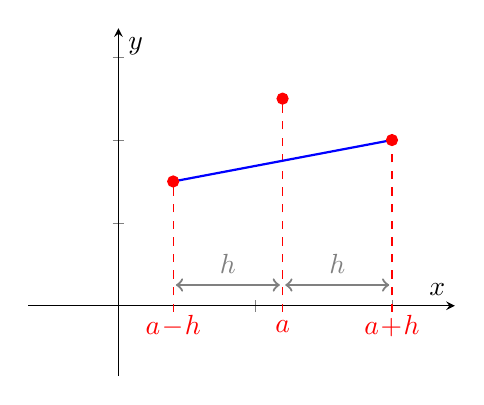
\begin{tikzpicture}
    \begin{axis}[
        legend pos=south east,
        axis x line=middle,
        axis y line=middle,
	xticklabels=\empty,
	yticklabels= \empty,
        grid = none ,
        width=7cm,
        height=6cm,
        grid style={dashed, gray!1},
        xmin=-2,     % start the diagram at this x-coordinate
        xmax=11,    % end   the diagram at this x-coordinate
        ymin=-1,     % start the diagram at this y-coordinate
        ymax= 6,   % end   the diagram at this y-coordinate
        xlabel=$x$,
        ylabel=$y$,
        enlargelimits=true,
        tension=0.08]

  \addplot[red, only marks, mark=*] coordinates {(2,3)(6,5)(10,4)};
  \draw [red,dashed] (axis cs: 2,-0.15) -- (axis cs: 2,3);
  \draw [red,dashed] (axis cs: 6,-0.15) -- (axis cs: 6,5);
  \draw [red,dashed] (axis cs: 10,-0.15) -- (axis cs: 10,4);
  \draw[blue,thick](axis cs: 2,3)--(axis cs: 10,4);
  \draw [<->,thick, gray] (axis cs: 2.1,0.5) -- (axis cs: 5.9,0.5);
   \draw [<->,thick, gray] (axis cs: 6.1,0.5) -- (axis cs: 9.9,0.5);
      

	\node(x0)[red] at (axis cs: 2,-0.5){$a \! -\! h$};
	\node(x1)[red] at (axis cs: 6,-0.5){$a$};
	\node(x2)[red] at (axis cs: 10,-0.5){$a \! +\! h$};
	\node(h1)[gray] at (axis cs: 4, 1){$h$};
	\node(h2)[gray] at (axis cs: 8, 1){$h$};
    \end{axis}
\end{tikzpicture}
\end{document}